\documentclass{standalone}
\usepackage{tikz}
\usepackage{xcolor}
\usetikzlibrary{circuits.ee.IEC}

\begin{document}
    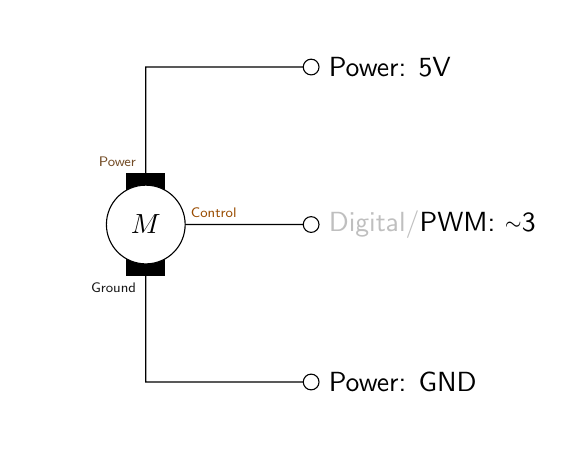
\begin{tikzpicture}[circuit ee IEC]
        % \draw[help lines] grid(10,10);
        \draw[draw=none,fill=white] (0.5,0.5) rectangle ++(6.5,5);


        \node[anchor=west,font=\sffamily] at (4.2,5) {Power: 5V};
        \node[anchor=west,font=\sffamily] at (4.2,3) {\textcolor{gray!50}{Digital/}PWM: {\raise.17ex\hbox{$\scriptstyle\mathtt{\sim}$}}3};
        \node[anchor=west,font=\sffamily] at (4.2,1) {Power: GND};

        \draw (4.1,5) circle(1mm) ++(-0.1,0) -- ++(-2,0) -- ++(0,-1.5);
        \draw (2,2.5) -- ++(0,-1.5) -- ++(2,0) ++(0.1,0) circle(1mm);% -- ++(0,-0.5) ++(0,-1.5) -- ++(0,-0.5) -- ++(2,0) ++(0.1,0) circle(1mm);
        \draw (2.5,3) -- (4,3) ++(0.1,0) circle(1mm);
        
        \node[anchor=east,font=\sffamily\tiny,text=black!40!brown] at (2,3.8) {Power};
        \node[anchor=west,font=\sffamily\tiny,text=black!40!orange] at (2.45,3.15) {Control};
        \node[anchor=east,font=\sffamily\tiny,text=black!90] at (2,2.2) {Ground};

        \draw[draw=none,fill=black] (1.75,3.4) rectangle ++(0.5,0.25);
        \draw[draw=none,fill=black] (1.75,2.6) rectangle ++(0.5,-0.25);
        \draw[fill=white] (2,3) circle(5mm);
        \node at (2,3) {$M$};
    \end{tikzpicture}
\end{document}         